\documentclass[lang=cn,11pt,a4paper]{elegantpaper}
\usepackage{url}
\usepackage{booktabs}
\usepackage{multirow}
\usepackage{geometry}
\usepackage{longtable}
\title{这整的啥玩意啊}
\author{万物主宰——王成航}
\date{2020.2}
% \usepackage[authoryear]{gbt7714}  % 国标

\begin{document}
\maketitle
\tableofcontents
\thispagestyle{empty}
\newpage
\pagenumbering{arabic}
\section{引言}
\subsection{当今的时代背景——大数据}
\par 早在20世纪末, 互联网便已经展现出了势不可挡的趋势, 随着互联网的迅速发展, 大数据成为了这个信息时代的标志词. 它的发展迅速到甚至可能我们连什么是大数据都不清楚, 就已经在生活的各个方面受到它的影响了. IBM提出大数据有5个特点, 分别是Volume、Velocity、Variety、Value、Veracity, 分别代表着大量、高速、多样、低价值密度和真实性. \figref{fig:data} 描述了近过去十年以及未来五年的数据量增长趋势, 可以很明显的看出数据量的增长目前还是呈指数形式. 这也意味着数据量的增长会犹如指数爆炸一般十分迅猛, 因此, 如何有效地利用如此海量的数据便是当务之急. 
\begin{figure}[htbp]
	\centering
	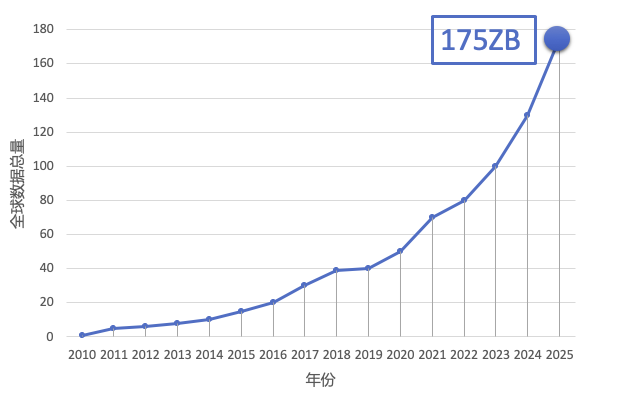
\includegraphics[width=0.6\textwidth]{Bigdata}
  	\caption{Rapid growth of data.\label{fig:data}}
\end{figure}
\par 由于对于数据处理的需求, 一些技术如"数据挖掘",、"机器学习"便被提了出来, 它们旨在运用现代强大的计算机和优秀的程序与算法. 对当今海量的数据进行处理, 从而找到一些有价值的信息. 随着数据量的大幅增大, 单台计算机已经无法满足数据处理的需要, 而以Hadoop为代表的开源分布式计算架构则提供了分布式计算的技术支持. 同时, 随着 Caffe 和 TensorFlow 等高效率的深度学习框架被开源,许多小型公司甚至个人也具备了自主研发改进算法和模型的能力. 互联网在不断发展,数据的生成也不会停下脚步. 
\par 如\figref{fig:data} 所示, 2020年全球数字宇宙将会已经超过50ZB, 虽然我们目前还不清楚这些数据如何被更加充分的利用, 不过可以肯定的是,数据会成为一项重要的资源,在大数据时代,特别是未来的智能化时代,如机器学习这种对于数据的处理技术一定会展现出更大的潜能. 正如马云所言, 人类社会的未来一定会进入数据处理技术(Data Technology,DT)时代.
\begin{figure}[htbp]
	\centering
	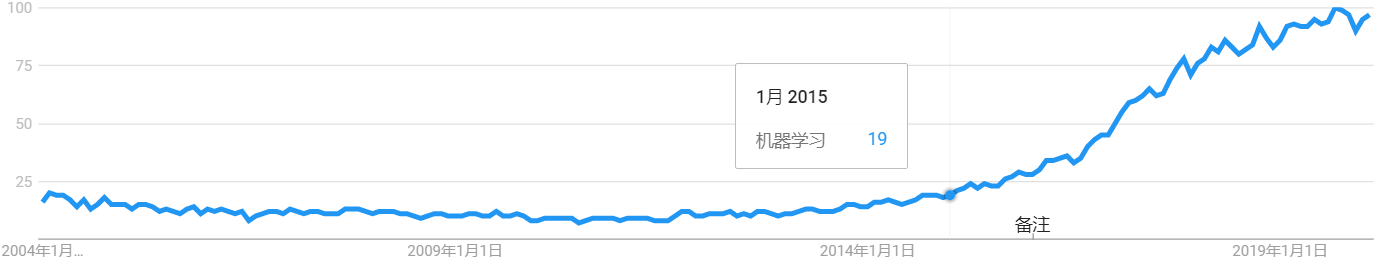
\includegraphics[width=0.7\textwidth]{GoogleTrend}
  	\caption{Google Trend about Machine Learning.\label{fig:GoogleTrend}}
\end{figure}
\par \figref{fig:GoogleTrend} 是"机器学习"这一词语在研究领域的谷歌搜索热度趋势\cite{GT}, 可以看出, 自2015年以来, 机器学习的搜索热度便急转直上, 这一结果可能要归功于Google旗下的DeepMind以及他们的AlphaGo. AlphaGo是一款通过机器学习构建出的围棋对弈系统, 其第一代系统于2015年3月与顶尖棋手李世乭进行了对弈, 并最终以3:1的大比分取得胜利. 经此一役, AlphaGo以及其背后的机器学习进入了大众的视野. 
\par 值得留意的是, 这项数据是从2004年开始的, 也就是说Google公司至少从2004年就开始不惜耗费十分巨大的财力与物力来保存这些来自全球的庞大的搜索数据了. 同样的, Facebook也在运用机器学习对每一个用户的每一条浏览记录, 每一次点赞进行分析, 从而为用户推送最为合适的内容以及广告. 国内公司对机器学习也有十分深入的应用, 如Alibaba的人脸支付, 能够在几亿用户中大规模正式上线人脸支付系统, 说明了Alibaba公司本身对于机器学习中人脸识别这一技术已经研发的十分完善. 而从2000年开始就有即时通讯业务的Tencent公司也将机器学习应用至很多产品, 如QQ中"可能认识的人", 或者音乐软件, 视频软件里可能喜欢的视频或者音乐, 里面都有机器学习的影子.
\par 类比于人脑的学习过程, 机器的学习似乎具有相似的性质, 人脑的学习过程(\figref{fig:Brian} )可以抽象为从经验之中总结出规律, 遇到新问题时基于过去总结而来的规律做出判断; 而机器学习的学习过程(\figref{fig:Machine} )则可以抽象为计算机从人为输入的历史数据中训练出模型, 对于新出现的的数据, 由已经训练好的模型给出预测. \figref{fig:AI}
\begin{figure}[htbp]
	\centering
	\begin{minipage}[t]{0.45\textwidth}
	\centering
	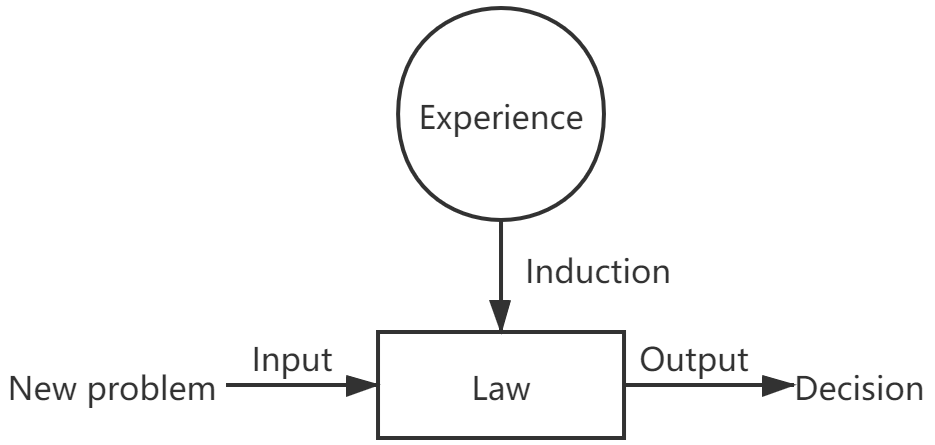
\includegraphics[width=1\textwidth]{Brian}
	\caption{How our brians learn.\label{fig:Brian}}
	\end{minipage}
	\begin{minipage}[t]{0.45\textwidth}
	\centering
	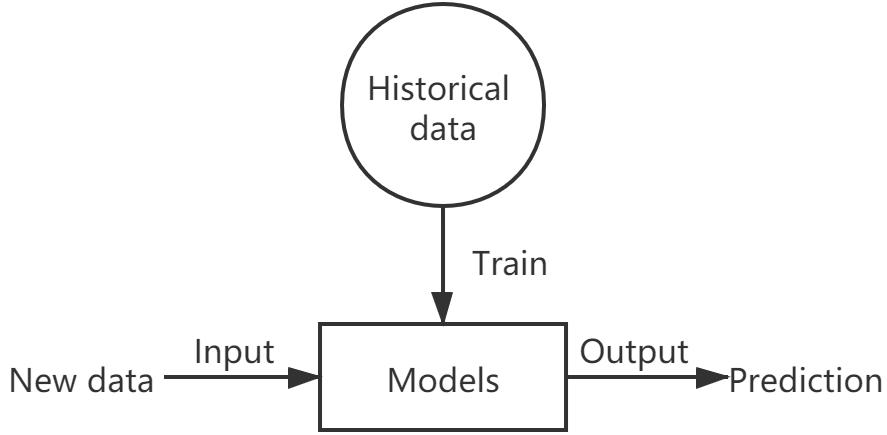
\includegraphics[width=1\textwidth]{Machine}
	\caption{How machines learn.\label{fig:Machine}}
	\end{minipage}
\end{figure}
\par 但机器学习本身却并不是一个十分年轻的事物, 它最早的应用可以追溯至1952年IBM工程师Arthur Samuel写出的一个跳棋程序, 这个程序通过学习走得好和不好的棋局, 为下棋者做出指导\cite{AS1}\cite{AS2}. 在过去的几年里, 机器学习、人工智能乃至深度学习都一度成为了资本投资的风口, 但其实此三者之间其实是包含与被包含的关系, 如同俄罗斯套娃一般(\figref{fig:AI} ).
\begin{figure}[htbp]
	\centering
	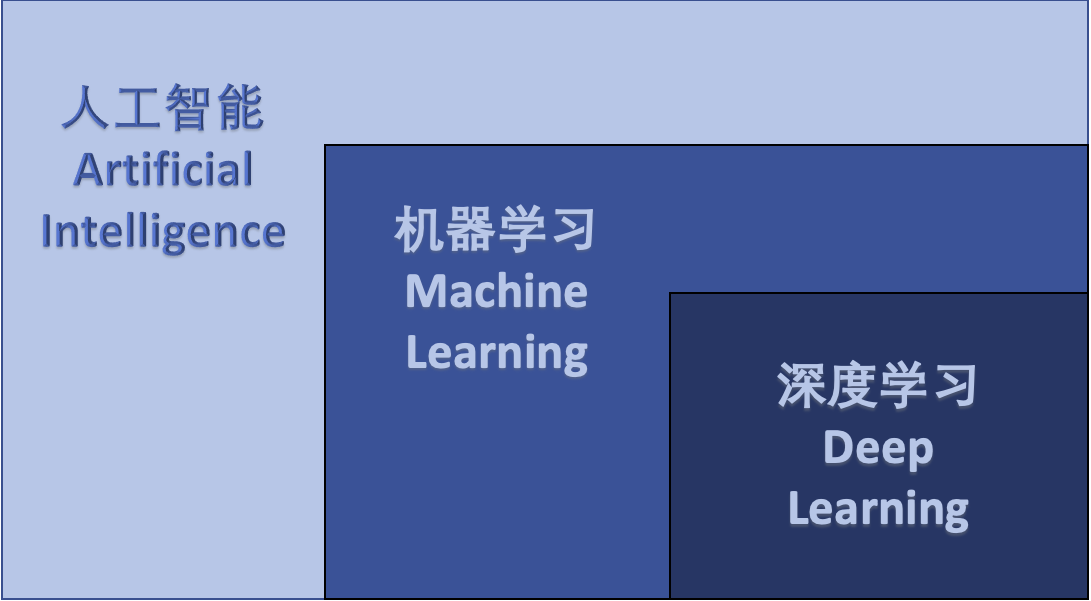
\includegraphics[width=0.6\textwidth]{AI}
  	\caption{AI, Machine Learning \& Deep Learning.\label{fig:AI}}
\end{figure}
\subsection{人工智能}
\par "人工智能"的概念自1956年在达特茅斯会议\cite{Dartmouth}上首次正式提出以来, 随着技术手段的发展也在不断地变化, 但它的核心是可以总结为"将由人类完成的智力任务自动化". 因此, 任何可以实现这一目标的手段与方法都可以冠以"人工智能"的名字. 
\par 但实现人工智能的方法并不仅限于机器学习, 例如早期的国际象棋程序Deeper Blue. 国际象棋的棋局复杂度($35^{80}$\cite{artic})并非特别庞大, 因此可以通过穷举法将每一种棋子走法都由程序编写后交给计算机进行计算, 而Deeper Blue通过这一方法成功地战胜了国际象棋世界冠军. 在Deeper Blue的下棋过程中, 不需要学习什么, 仅仅通过内置的程序进行计算即可. 这种通过编写复杂规则来实现人工智能的方法被称为符号主义人工智能. 
\par 但后来, 随着人们需要处理的信息越来越复杂, 如图像、音频或者是棋局复杂度十分巨大的围棋($250^{150}$\cite{artic}), 符号主义人工智能已经不能够处理这些问题了, 因此, 一种新的人工智能实现方法便出现了, 它便是"机器学习".
\subsection{机器学习}
\par 1950年, 人工智能先驱Alan Turing发表了"Computing machinery and intelligence"一文\cite{Turing2009}, .文中, 他对"计算机是否能够学习与创新"这一问题进行了思考, 并且给出了肯定的回答: 能. 
\par 经典的符号主义人工智能中, 我们输入的是数据以及精心编写的规则, 输出的是人们期望得到的答案(\figref{fig:old} ). 而在机器学习中, 输入的是数据和答案, 人们则希望计算机从这些数据与答案中学习到一些规则(\figref{fig:now} ). 
\begin{figure}[htbp]
	\centering
	\begin{minipage}[t]{0.45\textwidth}
	\centering
	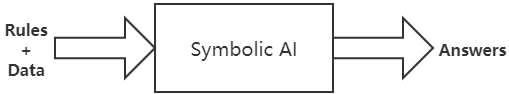
\includegraphics[width=1\textwidth]{Old}
	\caption{What Symbolic AI do.\label{fig:old}}
	\end{minipage}
	\begin{minipage}[t]{0.45\textwidth}
	\centering
	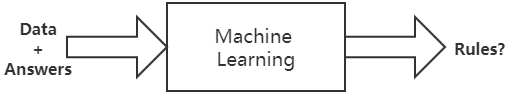
\includegraphics[width=1\textwidth]{Now}
	\caption{What ML do.\label{fig:now}}
	\end{minipage}
\end{figure}
\par 这一过程中, 计算机的学习系统是通过对输入数据以及对应的答案的观察来抽象出隐藏规则的. 到了现代, 甚至有许多问题我们只知道数据而不知道答案, 这时我们会只向计算机输入数据, 期待他能给我们答案, 这就是所谓的无监督学习. 事实表明, 一些并不借鉴人类输入数据的强化学习模型如AlphaGo Zero, 给出的答案甚至要比人类自己的答案好很多. 
\subsection{深度学习}
\par 在普通的机器学习问题中, 我们需要计算机去学习的规则,往往可以表达成输入数据的函数或者复合函数, 而在这些规则中有一部分的复合函数的复合次数甚至高达数十次乃至上百次, 对于这些复合函数十分复杂的问题, 我们称它们为深度学习问题, 深度学习的"深度", 便指的是这种多次复合函数的次数. 
\begin{figure}[htbp]
	\centering
	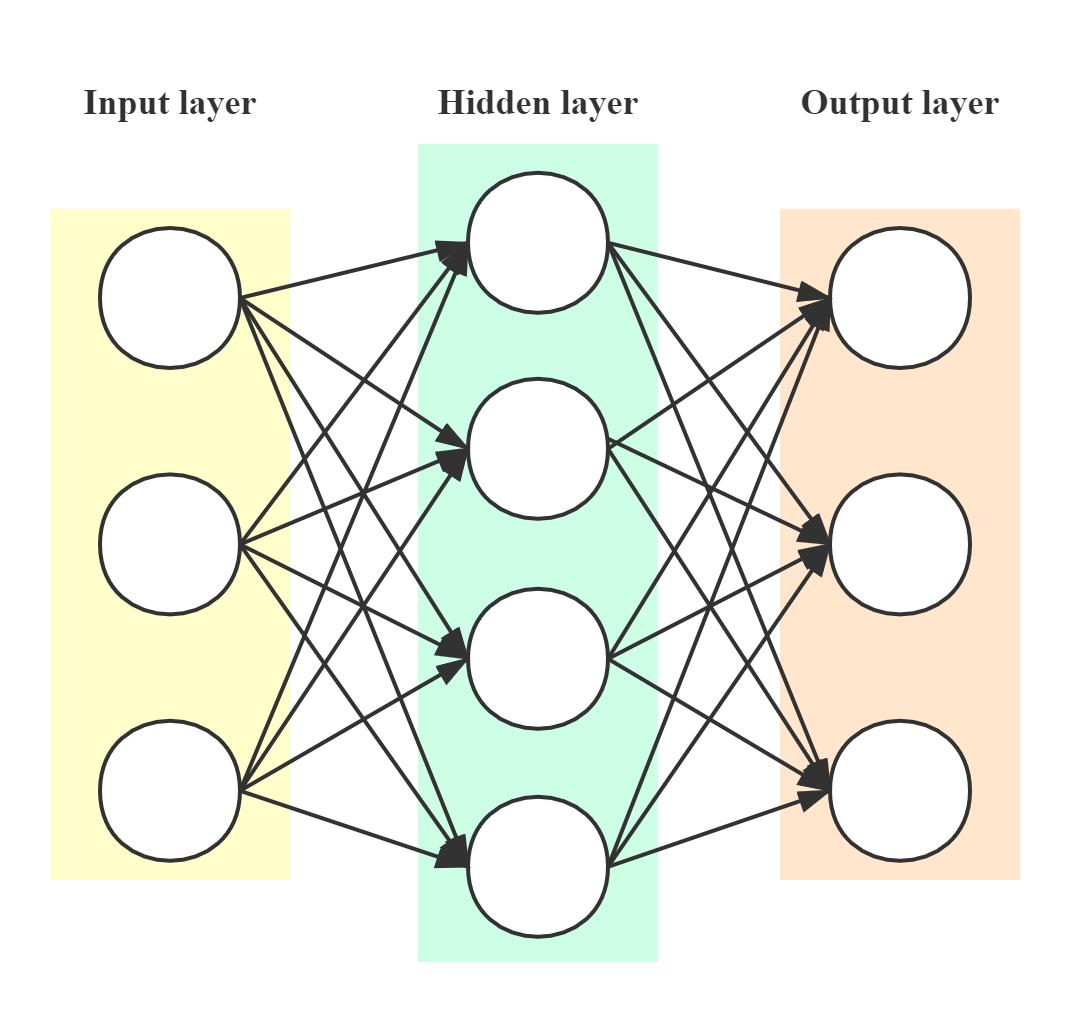
\includegraphics[width=0.6\textwidth]{DNN}
  	\caption{A three-layer full connected neural network\label{fig:DNN}}
\end{figure}
\par 而在实际的深度学习问题中, 这种多次的复合函数总是通过一种名叫"神经网络"的结构来实现的, \figref{fig:DNN} \cite{net} 便是一个三层的神经网络. "神经网络"这一术语的灵感来源于神经生物学. 虽然它的每一层十分简单, 但经过许多层的堆叠后, 往往可以对一些十分复杂的问题如图像识别等产生令人十分震惊的效果. 正像人的大脑虽然只由一个个细胞构成, 但却有十分复杂的智慧一样. 有监督的神经网络机器学习的基本原理如\figref{fig:net} , 它通过预测值与真实值的误差来调整自己每一层的参数, 使预测值变得更加精准.
\begin{figure}[htbp]
	\centering
	\hspace{-30pt}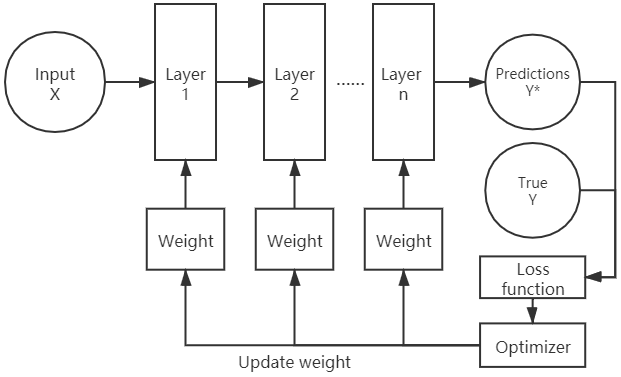
\includegraphics[width=0.6\textwidth]{Net}
  	\caption{The workflow of neural network ML.\label{fig:net}}
\end{figure}
\section{机器学习的发展与应用}
\subsection{发展历程}
\par 正如我们学习历史知识一样, 从机器学习的发展历史中了解它也是一种十分便捷的方式. 
\subsubsection*{20世纪50 - 70年代}
\par 此时, 人工智能正处于“推理期”,即人们用编程赋予机器逻辑推理能力,代表工作有: A. Newell和H. Simon的“逻辑理论家”( Logic Theorist )程序以及此后的“通用问题求解”( General Problem Solving )程序等,而他们二人也在之后获得了获图灵奖. 
\par 20世纪70年代中期开始,在E.A.Feigenbaum等的倡导下,人工智能研究进入了“知识期”,大量的专家系统问世. E.A.Feigenbaum等人也获得了图灵奖. 但是后来,知识工程也遇到瓶颈, 人们发现总结知识再教给计算机是相当困难的, 因此应该设法让机器自己学习知识.而图灵在1950年的文章中,肯定了机器学习的可能性;之后, 又陆续有基于神经网络的“连接主义”机器学习、基于逻辑表示的“符号主义”学习技术、以决策理论为基础的学习技术以及强化学习技术得到发展.
\subsubsection*{20世纪80年代}
\par 1986年,机器学习Machine Learning创刊;1989年,人工智能权威期刊Artificial Intelligence出版机器学习专辑;20世纪80年代机器学习成为一个独立学科领域, 同时, 各种机器学习技术也呈现着百花初绽的态势.
\par 此时的研究热门都聚集于"从样例中学习", 包括监督学习, 以及无监督学习. 其中, 以符号主义机器学习和基于神经网络的连接主义机器学习为主流, 前者包括决策树、基于逻辑的学习等, 后者虽然产生的是"黑箱"模型, 但由于能够有效地解决许多现实问题, 得到了广泛的应用.
\subsubsection*{20世纪90年代}
“统计学习”成为了这个年代的主流, 代表技术有支持向机SVM、“核方法”等.而统计学习事实上与连接主义学习关系密切,支持向量机被普遍接受后,核技巧(kernel trick)被广泛应用到机器学习各处,核方法逐渐成为机器学习基本内容.
\subsubsection*{21世纪}
"深度学习"成为了当代的主流, 以往的机器学习技术对使用者要求比较高,而相比于以往的机器学习技术,深度学习技术将对于使用者的高要求转移到模型的复杂度上了,以至于只要下功夫让计算机来调参,性能往往也不会很坏. 因此,虽缺乏严格的理论基础,但它显著降低了机器学习应用者的门槛,为其走向工程实践带来便利.
\subsection{应用实例}
\par 机器学习在当今其实已经“无处不在”,它普遍应用于人工智能的各个领域,包括数据挖掘、计算机视觉、自然语言处理、语音和手写识别、生物特征识别、搜索引擎、医学诊断、信用卡欺诈检测、证券市场分析、汽车自动驾驶、军事决策等.
\paragraph{异常检测}异常指的是某个数据对象由于测量误差、收集中的损失或自然变异等原因变得不同于正常的数据的场景,而将这些异常辨别出的过程,通常称为异常检测. 异常检测的训练样本都是非异常样本,假设这些样本的特征都是服从高斯分布,则在此基础可以建立一个概率模型,用来估计就有某个特征的样本属于非异常样本的可能性. 比如当用户的信用卡发生了一笔特征与平常的交易的特征不同的交易请求时, 就有可能是信用卡被盗刷, 这是银行就可以根据风控系统来防止这样的盗刷发生.
\paragraph{用户画像}用户画像的核心工作就是给用户打标签,如年龄、性别、地域、兴趣等. 公司从这些标签集合能抽象出一个用户的信息全貌. 从而在产品的运营和优化中,根据用户画像深入理解用户需求,从而设计出更适合用户的产品,设定复合用户消费能力的价格区间, 提升用户体验等. 现在的各个APP对于用户的个性化推荐、支付宝的芝麻信用分等都属于用户画像的具体应用.
\paragraph{广告点击率预估}互联网广告是互联网公司主要的盈利手段,当今的科技巨头Google便是以广告为主业. 互联网广告交易的双方是广告主和媒体. 为自己的产品投放广告并为广告付费;媒体是有流量的公司,如各大门户网站、各种论坛,它们提供广告的展示平台,并收取广告费. 广告点击率是指广告的点击到达率,即广告的实际点击次数除以广告的展现量. 在实际应用中,我们将海量的历史点击数据作为样本来训练模型,从而评估各方面因素对点击率的影响. 作为这一模型的应用, 当有新的广告位请求到达时,就可以用训练好的模型,根据广告交易平台传过来的相关特征预估这次展示中各个广告的点击概率,结合广告出价计算得到的广告点击收益,从而选出收益最高的广告向广告交易平台出价. 
\section{统计学跟机器学习的对比}
\par 传统统计学统计与机器学习都是通过现有的数据预测或是还原一些关系的学科. 
\par 机器学习是目标驱动的, 为了解决在其他领域里遇到的挑战与困难, 不断地改进现有的方法或者提出新的想法. 最终目标是不断地更好地解决实际问题. 并且已经成功地在目标识别, NLP, 人机对弈等等领域里取得了传统统计学无法想象的成就. 人们想到机器学习的时候想到的不是一个一个数学定理, 而是机器学习所解决的这些关键的问题. 
\par 传统统计学, 在解决问题的同时也更多的注重于理论的完备性, 解决问题并且解释问题. 传统统计学的发展往往依赖并推动着随机矩阵, 随机过程, 泛函分析与几何学等应用数学甚至纯数学等领域里的的新方法的提出. 我们想到统计学的时候往往想到的是各种各样的统计方法以及这样的我们对这样的方法所能做出的评价.
\par 同样一个问题在传统统计学与机器学习的视角下可以有这极大的研究方向的不同. 比如推荐系统. 根据用户的观看数据去预测用户的喜好从而达到给用户推荐新的电影小说或者是商品的这样一个任务. 机器学习跟传统统计学相比可能就有着完全不同的解决问题的途径.
\subsection{机器学习视角-回归模型}
\par 在机器学习的视角下, 一种最简单的办法是训练出一套回归系统$f:\mathcal X \to \mathcal Y$, $\mathcal X \subset \mathbb R^m, \mathcal Y \subset \mathbb R^n$, 对一个用户的年龄性别地址打分记录等一系列可能对电影喜好有影响的数据, 用特征提取的方法提取出来一个用户的特征$x\in \mathcal X$, 将其输入网络, 就可以输出一个代表着他所喜爱的电影的相应特征$y\in \mathcal Y$, 比如经过特征提取后的电影发布的时间, 电影的种类与电影的描述、影评电影的相关信息等等. 然后通过对所有电影库里的电影进行特征提取, 取最相近的一个, 我们就可以找到最合观众口味的电影.
\par 在这个过程里, 我们假定这样的用户的特征跟电影的特征之间存在着某种高度非线性关系, 并且机器学习让我们可以近似出这样的高度非线性的关系, 比如用最简单的Deep ReLU Network(当然真的可不可以我没试过). 
在海量用户观看数据的支持下, 设置好用户跟电影特征提取过程中的参数与学习率、网络深度、每一层神经元数等一系列超参数, 在训练集$E\in \mathcal X \times \mathcal Y$上对性能度量$||f(x)-y||^2_2, (x,y)\in E$做随机梯度下降, 用已经很成熟的反向传播算法就可以把网络优化得很好. 这个时候我们就已经的到了一个从用户特征空间$\mathcal X$到电影特征空间$\mathcal Y$的一个映射, 通过上面的步骤我们也就获得了一个最简单的电影推荐系统. 因为没有做过实验, 我们不对这一小节里的内容的严谨性负责, 但是对于更先进的推荐系统可以参考协同过滤算法\cite{Goldberg1992}.
\par 如果我们采用与机器学习同样的思路去尝试用传统统计学解决这个问题, 这样的实际问题中的高度非线性性给传统统计学带来了巨大的困难. 并且对于这种实际问题尽管我们知道他们相关, 可我们根本不知道这样的相关函数具体属于什么样的函数空间或者函数类, 这使得非参方法的合理性无法保证. 甚至就算我们知道了他属于哪些函数空间, 函数空间无穷维的特性也使得我们失去了有限维情况下的很多概率工具. 在这个具体的例子里面, 问题主要还是出在我们无法找到任何一个具体的函数类去合理地为这种特征与特征间非线性的关系建模. 基本上所有的假设都能自圆其说, 也就使得这些假设都失去了实际意义.
\par 传统统计学在十年前已经对这样一个问题给出了一个十分漂亮优雅的答案\cite{Candes2010} , 并且由此使用的与发展出的方法都具有启发性. 
\subsection{传统统计学视角-矩阵补全}
\par 矩阵补全, 简单来说就是对于一个巨大的矩阵$A\in \mathbb{R}^{n_1\times n_2}$, 凭借我们所知道的其中一部分元素能否复原整个矩阵? 当然在不加任何假设的情况下, 这样一个问题不管用什么方法都是不可能的. 因为我们不知道任何关于这个矩阵的其他信息. 不过在我们知道了关于一个矩阵的其他信息比如这个矩阵低秩\cite{Candes2010}或者列空间可分为低维空间的并\cite{Eriksson2012}, 这个问题便有了一定的可解性. 并且如果这个矩阵满足了一定限制, 我们可以给出一个精确的补全\cite{Candes2009}.
\par 在这个应用场景下低秩是一个相对宽松但是又有一定合理性的假设, 因为在实际情况中往往少数因素就可以决定用户的喜好\cite{Candes2010}. 这样一个矩阵$A$可以代表着用户对所有电影的潜在的喜好程度, 其元素$X_{i,j}$代表第i个用户对j个商品的喜好程度, 假设$rank(X)=r, r<<n$. 但是我们并没有对$A$的直接观测, 因为并不是每个用户都能接触到所有的商品并写出反馈. 所以我们实际上的观测只局限于在这个确定矩阵的元素里随机抽取其中的m个. 记我们观测到的矩阵为矩阵$Y\in \mathbb{R}^{m\times n}$,
\begin{equation}
	Y_{ij}:=\delta_{ij}X_{ij}, \quad \delta_{ij} \sim \text{Ber}(p) \text{ are independent}, \quad p=\dfrac{m}{n_1n_2}
\end{equation}
\par 我们希望能够最好的复原这样的矩阵, 最好的意思是复原出的矩阵$\hat{X}$能够使得$||\hat{X}-X||_F$最小. (注意这里虽然我们假设了$X$低秩但是观测到的矩阵$Y$不一定低秩).
\par 统计学理论可以证明这样的矩阵补全可以被矩阵$p^{-1}Y$的最佳r阶逼近所达成\cite{Recht2011}. 其中最佳r阶逼近可以写作
\begin{equation}
	p^{-1}Y_r=\frac{1}{p}\sum_{i=1}^r s_i u_i \otimes v_i, s_i \in \mathbb R, u_i \in \mathbb R^{n_1}, v_i\in \mathbb R^{n_2}
\end{equation}

即对矩阵$Y$的谱分解在第r个奇异值处截断, 最佳指的是 
\begin{equation}
||Y_r-Y||=\min_{rank(Y')\leq r}||Y-Y'||,
\end{equation}
其中对 $||\cdot||$ 任意的酉不变范数, 包含F范数与2-范数, 这样最佳逼近的求解实际上等价于一个凸优化问题. 那么这样的$\hat X$不但可以作为矩阵补全的一个方式, 并且统计学还给出了它的性能能够达成到一个什么样的程度?
\par 统计学的理论可以证明, 只要我们知道的元素够多, 多到$m\geq ctn\log n,\, n=\max\{n_1,n_2\}$的时候, 我们就很有可能(概率大于$1-(2n)^{1-t}$)能让估计误差变得很小
\begin{equation}
	\dfrac{1}{n}||\hat X -X||_F\leq C\sqrt{\dfrac{tn\log n}{m}}||X||_{\infty},
\end{equation}
 其中$t>1$, $c,C$是两个不依赖于$X$的参数\cite{Recht2011}. 
 
 \par 并且更进一步, 统计学的理论可以证明, 对于一些稍微更特殊的矩阵($A$的左右特征向量组是两组正交向量组), 只要我们观测到的元素数量够多, 多到$m\geq C n^{1.2} \log(n)$, 我们就很有可能(大于$1-cn^{-3}\log n$), 我们能够精准的补全$A$, 其中$c,C$是两个不依赖于$X$的参数\cite{Candes2009}. 再进一步, 统计学的理论还可以证明, 这样的Completion是近乎最完美的, 因为他接近了信息论所允许的不可能再提升的下界(差一个$\log n$)\cite{Candes2010}.
\par 这是为数不多的统计学理论几乎能与机器学习在实战中相媲美, 同时又给出很漂亮理论解释的场景. 但是就在这样的场景下我们也可以看出他们研究风格的巨大区别. 在更多的场合里, 机器学习的前沿发展在一些项目上已经使人类高手相形见绌, 而统计学理论解释机器学习的分支却还处在婴儿阶段. 
\par 机器学习突破了传统统计学在数学严谨性要求上的枷锁, 本着黑猫白猫抓住了老鼠就是好猫的精神不断地在工程上取得了一个又一个惊人的突破. 同时机器学习也对传统统计学理论的发展提供了新的方向与灵感, 比如研究网络结构的Expressiveness\cite{Yarotsky2017}以及学习过程的Empirical Process\cite{Vapnik1994}的探索等等, 而这些催生出的统计理论在量子物理、数据科学等方向的再次应用也远远超出了机器学习或是人工智能的范畴.

\section{机器学习的未来展望}

贯穿整个深度学习的发展历史, 不管是逻辑启发的符号主意还是生物学启发的链接主意, 其已经将人类文明带到了新的高度. 但是它也遇到了很多无法破除的限制. 那么现在机器学习面临的困难有哪些?未来的发展方向又在哪里? 这是一个远远超出了我们能回答范围的问题, 不过Hinton和LeCun在2019年图灵奖颁奖时的讲话也许能给我们些许的灵感.

首先Hinton认为\cite{Youtube}在计算机视觉的领域, 对于目标识别任务, 我们目前的神经网络认知的方式与我们人认知的方式并不一致. 人类可以利用并且依赖于的各个部件之间的几何关系, 在视角变换下的不变关系, 来认知事物, 而神经网络往往忽视了这一点. \cite{kosiorek2019stacked}

其次我们在神经网络里只有两种时间尺度, 一种缓慢的权重适应, 一种激活的神经元的快速变化. 这与生物学上神经元所具有的有适应各种时间尺度变化的能力有所差距. 所以一个方向时能够引入一些更多的时间尺度, 使得神经网络更迅速地对权重完成调整, 实现对短期记忆的快速重建. 

虽然我们身处大数据时代, 但是有一些数据依然是无法获得的. 比如虚拟世界中表现优异的强化学习在现实应用中往往因为无法接受的数据成本(比如自动驾驶)而发展受阻. 毕竟我们不能为了收集每一个样本就撞一次车, 或是摔坏一个机器人, 尽管这样的成本在虚拟场景下比如游戏里面是唾手可得的. 但是我们的纯粹的强化学习却需要大量这样的数据去完成学习. 或者我们需要更多的数据, 或者我们需要改变我们的策略.

LeCun认为机器学习的未来在自监督学习与半监督学习. 因为对于纯强化学习而言网络被输入的关于每个样本的有效信息往往是很少的, 像是蛋糕上的樱桃. 对于监督学习而言这个信息量就比较巨大, 像是蛋糕上面的冰层. 而对于自监督学习而言这些单个样本提供的信息量就更为巨大, 像是真正的蛋糕. 这个世界不是完全可预测的, 也不是完全随机的, 所以在有限的样本下, 我们需要尽可能多的信息去克服这样的不确定性.

最后, 对智能的理论依旧是空缺, 机器学习理论或者人工智能理论在未来会如何挑战我们对自己与对机器学习的认知?而这些理论上的突破又会如何知道我们的发明与创造? 这些事情都值得我们期待.

\section{机器学习基本步骤}
机器学习虽然是一门具体理论比较复杂的学科, 但其基本步骤却可以高度简单的抽象出来, 下文就简单介绍一下典型的机器学习中的几个步骤.
\subsection{数据获取与预处理}
所有机器学习算法尽管有各方面的不同, 但大都有一点是相同的——都是数据贪婪的,即任何一个算法,都可以通过增加训练数据来达到更好的结果. 因此我们的首要工作便是获得尽可能多的有效的数据. 在获得数据集之后,进行数据清洗、数据预处理、以及特征选择、降维等工作, 而这些预处理, 特征选择, 降维等工作都是为了模型可以更好地来学习数据.
\subsection{模型选择}
在模型中, 一般有三个需要人为选定的参数, 它们是决策函数集、目标函数( 表现度量 )和优化算法.
\paragraph{决策函数集}即要选定使用什么样的函数集合来构建模型.
\paragraph{目标函数( 表现度量 )}即需设定衡量决策函数好坏的度量方法.
\paragraph{优化算法}即使用什么样的算法根据表现度量来对决策函数中的参数进行优化. 
\newpage
\appendix
\pagenumbering{Roman}
\section{机器学习的发展历程}
\begin{longtable}[c]{|l|l|l|}
	\hline
	年份    & 事件                                                                                                               & 时期                                                                      \\ \hline
	\endfirsthead
	%
	\endhead
	%
	\hline
	\endfoot
	%
	\endlastfoot
	%
	1949年 & Hebb基于神经心理学提Hebb学习规则                                                                                             & \multirow{6}{*}{\begin{tabular}[c]{@{}l@{}}基础奠定的\\ 热烈时期\end{tabular}}   \\
	1950年 & Alan Mathison Turing创造了图灵测试                                                                                      &                                                                         \\
	1956年 & \begin{tabular}[c]{@{}l@{}}John McCarthy, Cloude Shannon等人\\ 提出“人工智能 ( Artificial Intelligence )”\end{tabular}   &                                                                         \\
	1957年 & \begin{tabular}[c]{@{}l@{}}Frank Rosenblatt设计出了第一个\\ 计算机神经网络——感知机 (The Perceptron )\end{tabular}                 &                                                                         \\
	1956年 & \begin{tabular}[c]{@{}l@{}}Arthur Samuel发明“机器学习”( Machine Learning )这个词, \\ 并以他开发的西洋跳棋程序打败了当时的西洋棋大师\end{tabular} &                                                                         \\
	1967年 & k最近邻分类算法( KNN )出现                                                                                                &                                                                         \\ \hline
	\multicolumn{3}{|c|}{停滞不前的冷静时期:20世纪60年代中叶到70年代末}                                                                                                                                                   \\ \hline
	1980年 & \begin{tabular}[c]{@{}l@{}}卡内基梅隆大学( CMU )召开了\\ 第一届机器学习国际研讨会\end{tabular}                                         & \multirow{4}{*}{\begin{tabular}[c]{@{}l@{}}重拾希望的\\ 复兴时期\end{tabular}}   \\
	1984年 & Breiman等人提出分类与回归树( CART )                                                                                        &                                                                         \\
	1986年 & 国际性杂志\emph{Machine Learning}创刊                                                                                          &                                                                         \\
	1986年 & \begin{tabular}[c]{@{}l@{}}Rumelhart和McClelland为首的科学家\\ 提出BP神经网络\end{tabular}                                    &                                                                         \\ \hline
	1989年 & \begin{tabular}[c]{@{}l@{}}Yann LeCun在贝尔实验室就开始使用\\ 卷积神经网络( CNN )识别手写数字\end{tabular}                              & \multirow{6}{*}{\begin{tabular}[c]{@{}l@{}}现代机器学习的\\ 成型时期\end{tabular}} \\
	1995年 & Vladimir Vapnik提出支持向量机( SVM )                                                                                    &                                                                         \\
	1995年 & Freund和schapire提出了 AdaBoost算法                                                                                    &                                                                         \\
	1997年 & 循环神经网络( RNN )提出                                                                                                  &                                                                         \\
	2000年 & \begin{tabular}[c]{@{}l@{}}流形学习方法( Manifold Learning )在\\ \emph{Science}上被提出,现代应用包含Isomap、LE、PCA\end{tabular}           &                                                                         \\
	2001年 & Breiman提出随机森林( Random Forest )                                                                                   &                                                                         \\ \hline
	2006年 & \begin{tabular}[c]{@{}l@{}}Hinton等人在\emph{Science}上提出了一种\\ 训练深层神经网络的方法\end{tabular}                                     & \multirow{7}{*}{\begin{tabular}[c]{@{}l@{}}大放光芒的蓬勃\\ 发展时期\end{tabular}} \\
	2010年 & Leslie Valiant因PAC理论获得图灵奖                                                                                        &                                                                         \\
	2011年 & Judea Pearl因概率图模型获得图灵奖                                                                                           &                                                                         \\
	2012年 & \begin{tabular}[c]{@{}l@{}}Hinton小组发明的深度卷积神经网络\\ AlexNet首先在图像分类问题上取代成功\end{tabular}                              &                                                                         \\
	2014年 & Lan.J.Goodfellow等人提出GAN                                                                                          &                                                                         \\
	2017年 & AlphaGo战胜柯洁                                                                                                      &                                                                         \\
	2019年 & \begin{tabular}[c]{@{}l@{}}Geoffrey E Hintion、Yann LeCun、Yoshua Bengio\\ 因在深度学习方面的贡献获得图灵奖\end{tabular}           &                                                                         \\ \hline
	\end{longtable}
\newpage
\nocite{*}

% 如果想修改参考文献样式(非国标),请把下行取消注释,并换成合适的样式(比如 unsrt,plain 样式). 
\bibliographystyle{unsrt}
\bibliography{wpref}

\end{document}
